\documentclass[tikz,border=10pt]{standalone}
\begin{document}
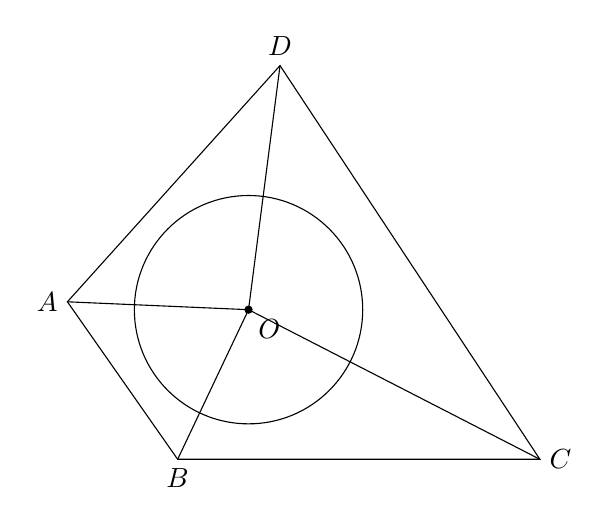
\begin{tikzpicture}[scale=1]
  \coordinate (A) at (0,2);
  \coordinate (B) at (1.4,0);
  \coordinate (C) at (6,0);
  \coordinate (D) at (2.7,5);
  \coordinate (O) at (2.3,1.9);

  \draw (A) -- (B) -- (C) -- (D) -- cycle;
  \draw (O) circle (1.45);
  \draw (A) -- (O);
  \draw (B) -- (O);
  \draw (C) -- (O);
  \draw (D) -- (O);
  \fill (O) circle (1.5pt);

  \node[left] at (A) {$A$};
  \node[below] at (B) {$B$};
  \node[right] at (C) {$C$};
  \node[above] at (D) {$D$};
  \node[below right] at (O) {$O$};
\end{tikzpicture}
\end{document}
